% !TEX root = paper.tex

\section{Introduction}
\label{s:intro}

\begin{figure*}
\centering
\includegraphics{fig/overview}
\caption{\name's architecture, made up of two parts: a {\em database
    proxy} and an unmodified {\em DBMS}, which uses
  user-defined functions (UDFs) to implement components of \name{}.
  Rectangular and rounded boxes represent processes and data,
  respectively.  Shading indicates components added by \name.  Dashed
  lines indicate separation between users' computers, the application
  server, and the DBMS server.  \name{} addresses two kinds of
  threats, shown as dotted lines.  In threat 1, a curious database
  administrator with complete access to the DBMS server snoops on
  private data, in which case \name{} leaks no data.  In threat 2, an
  adversary gains {\em complete} control over both the software and
  hardware of the application and DBMS servers, in which case
  \name{} leaks no data of currently inactive (not logged in) users
  (data of user 1 in this example may leak).}

\label{fig:overview}
\end{figure*}

% \nz{Today: no privacy guarantees if application/server/database are
% compromised.  This paper is about how to provide some privacy guarantees
% in the face of arbitrary server compromises.  Need to compare briefly
% to apps that either don't trust the server (SPORC, Depot), or that
% don't need a server: Ivy~\cite{muthitacharoen:ivy}, peer-to-peer apps:
% not all apps can be distributed across clients, and even when possible,
% it's difficult to do for existing server-side applications.}

Theft of private information is a significant problem, particularly
for online applications~\cite{prc:breaches}.  An adversary can exploit
software vulnerabilities~\cite{cve:stats} and bugs to
gain unauthorized access to servers; curious or malicious
administrators at a hosting or application provider can snoop on
private data~\cite{chen:gmail-snooping}; and attackers with
physical access to servers can cause significant
damage~\cite{halderman:cold-boot}.

%Although an impressive amount of work has gone
%into preventing compromises in the first place, vulnerabilities and
%attacks remain commonplace~\cite{prc:breaches,cve:stats}.

One approach to reduce the damage caused by server compromises is to
encrypt sensitive data, as in SUNDR~\cite{li:sundr},
SPORC~\cite{feldman:sporc}, and Depot~\cite{mahajan:depot}, and run
all computations (application logic) on clients.  Unfortunately,
several important applications don't lend themselves to this approach,
such as a database-backed web site that processes queries to generate
data for the user, or an application that computes over large amounts of data.  Even when this approach is
tenable, converting an existing server-side application to this form can be
difficult.  On the other hand, one might consider theoretical solutions such as fully-homomorphic
encryption~\cite{gentry:fhe} to allow servers to compute over
encrypted data.  However, these schemes are currently wildly
impractical, with slowdown estimates on the order of a trillion
times~\cite{trillion}.

This paper presents \name{}, a system that explores an intermediate
design point to provide practical privacy guarantees for applications
that use database management systems (DBMSs).  \name leverages the
typical structure of database-backed applications, consisting of a
DBMS server and a separate application server, as shown in
Figure~\ref{fig:overview}; the latter runs the application code and
issues DBMS queries on behalf of different users.  \name's main idea
 is to {\em execute queries over encrypted data} and the key insight
that makes it practical is that SQL uses a well-defined set of
operators, each of which we are able to run over
encrypted data.

\name{} addresses two threats.  The first threat is a {\em curious
  database administrator} (DBA) who tries to learn private data (e.g.,
health records, financial statements, personal information, etc.) by
snooping on the DBMS server; here, \name ensures that the DBA cannot
extract any private data.  The second threat is an {\em adversary that
  gains complete control of application and DBMS servers}.  In this
case, \name cannot provide any guarantees for users that are logged-in the application during an attack, but still guarantees the confidentiality of
other users' data.

% In this paper, we consider a design point between ``no server
% computation'' and ``arbitrary server computation'': {\em perform SQL
% query execution over encrypted data}.  SQL relational databases are
% widely used and perform non-trivial (though not entirely arbitrary)
% computations.

% We present {\em \name{}}, a practical system that executes SQL queries
% and transactions over encrypted data without decrypting the data to a
% clear-text format, providing strong privacy guarantees in the face of
% server compromises.  With \name{}, the DB server is entirely
% untrusted, and application servers are trusted only with respect to
% the private data of principals---e.g., web application users---who are
% currently logged in.

% Database management systems (DBMSs) are
% an especially appealing target for attackers, because they often
% contain large amounts of private information.  When individual
% users or enterprises store their sensitive data in a DBMS today, they
% must trust that the server hardware and software are uncompromisable,
% that the data center itself is physically protected, and assume that
% the system and database administrators (DBAs) 
% %who maintain the DBMS software 
% are trustworthy.  Otherwise, an adversary who gains access to any of
% these avenues of attack can compromise the entire database, as has
% been documented in a number of published reports of data
% thefts~\cite{prc:breaches} (and presumably there are more
% compromises that have not been publicized).

% These stringent security requirements are also at odds with
% cost-saving measures such as the consolidation of DBMSs belonging to
% different business units into a common enterprise-wide IT
% infrastructure, moving databases into a public cloud, or outsourcing
% DBA tasks.  In fact, ``lack of trust'' is an oft-quoted primary
% concern about moving data in database systems to more cost-effective
% cloud infrastructures.  Moreover, thanks to high-profile thefts of
% social security identifiers, credit card numbers, and other personal
% information from various online databases, these concerns are
% increasingly being reflected in the law as well: for instance, recent
% legislation requires that all databases containing personal data about
% Massachusetts residents be encrypted~\cite{Masslaw}.



% A significant barrier to deploying database systems in the cloud is
% the perceived lack of privacy, which in turn reduces the degree of
% trust users are willing to place in such deployments. If clients were to
% encrypt all the data stored in the cloud database, and if the data
% were decrypted only on client-controlled machines, then privacy
% concerns would largely be eliminated. Similarly, even in so-called
% private clouds inside enterprises, users often desire the ability to
% store data and run queries in data centers without trusting the
% database and system administrators with the content.

%In \name, unmodified DBMS servers store {\em all} sensitive data in
%an encrypted format, and execute SQL queries over encrypted data without
%having access to the decryption keys.  

% \hb{May not be necessary for SIGMOD.}
% SQL provides a good trade-off between generality and efficiency in cloud storage.
% On the one hand, SQL is widely used and useful to the many applications that
% already store their data in SQL databases, and use SQL queries to efficiently
% process their data.  On the other hand, SQL provides a structured data
% representation and a declarative query language that is much easier to reason
% about and to process efficiently over encrypted data than a general-purpose
% computation.


% \hb{Less related work here.}
% While early proposals attempted to enable SQL processing over encrypted
% data~\cite{sqlOverEncryption}, their privacy mechanisms were mostly heuristic,
% required a significant rewrite of the DBMS design, relied on considerable
% client-side processing, and did not support certain SQL queries. More recent
% literature~\cite{Dawn-Song-Search-2000, Chang04privacypreserving,
% queriesEncryptionBoneh,
% amanatidis-boldyreva-o'neill, Yang-privacy-preserving-queries,
% encrypt-for-secure-outsource, private-query-multi-user-for-searchable} has
% developed cryptographic tools for searching keywords on encrypted data and has
% proposed using these tools to process SQL queries on encrypted data. Although such
% work is a good first cut at the problem, it does not provide a
% comprehensive systems solution: they do not support many basic SQL queries (and
% mostly only support equality comparisons), some of them require significant
% client-side query processing, change the internal processing of a DBMS, and many
% of these schemes are too inefficient (requiring users either to build and maintain
% indexes or to perform sequential scans for every selection).

There are two challenges in combating these threats.  The first lies
in minimizing the amount of data revealed to the DBMS server, without
sacrificing the ability to execute queries efficiently.  Using
a single key to encrypt each row in the database would not allow the
DBMS server to execute many SQL queries without access to the
decryption key; consider, for instance, a query that asks for the
average salary of employees or for the names of employees whose salary
is greater than \$60,000.  These queries require computing over
encrypted data, but existing approaches that provide this capability
are either too slow for real-world use or don't provide adequate
confidentiality.  An ideal solution should impose a low performance
overhead on the DBMS server, avoid executing queries outside the DBMS,
and run on unmodified DBMS server software to benefit from decades of
engineering effort in optimizing DBMS performance.

%Moreover, a practical solution would operate not
%require DBMS software changes, to take advantage of decades of
%engineering and optimization work.

The second challenge is to minimize the amount of data leaked when an
adversary compromises the application server.  An ideal solution would
ensure that the application can issue queries only for data it
legitimately requires, and not for arbitrary data requested by an
adversary.  However, this task is difficult because the DBMS server
can also be subverted by the attacker, so \name cannot trust it to
prevent the application from reading arbitrary data.  Moreover, the
application itself has legitimate access to \name{}'s decryption keys,
and assigning each user a different database encryption key is
inadequate for applications with shared data, such as a bulletin board
or a conference review site.

%that gains access to the database and application servers can subvert
%both of them.

% \nz{Do we really need this challenge?}  \hb{I think we should rewrite
%   this challenge somehow to get at the adjustable encryption solution:
%   i.e., somehow say that there might be the equivalent of ``the
%   minimum required information'' to process a query and we want to get
%   that.}  

% The third challenge is in designing a system that balances the need
% for server-side computation with the need to minimize information
% revealed to the untrusted DB server.  An ideal solution would reveal
% only the smallest amount of information about the data required to run
% any given query mix.

% The third challenge is to carefully define ``privacy'' for
% an untrusted DBMS, as well as come up with a system design that
% provably achieves that definition.  On the one hand, even if all of
% the data stored on a DBMS server were encrypted, the server must be
% able to perform certain operations on the rows, such as aggregations,
% selections, and joins.  On the other hand, an adversary that
% compromises a DBMS server may now learn information about the data,
% such as relations between different rows in a table.  Thus, we need to
% define privacy in a way that balances the need for server-side
% computation with the need to minimize information revealed to the
% server.

\name{} addresses these challenges using three novel ideas.  The first
is to {\em execute SQL queries over encrypted data}.  \name{}
implements this idea using an {\em SQL-aware encryption strategy},
which leverages the fact that all SQL queries are made up of a
well-defined set of primitive operators, such as equality checks,
order comparisons, aggregates (sums), and joins.  By adapting known
encryption schemes (for numeric and string equality, additions, and
order checks) and using a new privacy-preserving cryptographic method
for joins, \name{} encrypts each data item in a way that allows the
DBMS to execute on the transformed data.
%For example, to perform
%equality checks over encrypted data, \name encrypts data with a
%deterministic encryption scheme, so that equal plaintexts have equal
%ciphertexts.  
\name{} is efficient because it mostly uses symmetric-key encryption,
avoids fully-homomorphic encryption, and runs on unmodified DBMS
software (with user-defined functions).

Some encryption schemes leak more information about the data to the
DBMS server than others, but are required to process certain queries.
To avoid revealing all possible encryptions of data to the DBMS {\em a
  priori}, \name carefully {\em adjusts} the SQL-aware encryption
scheme for any given data item, depending on the queries observed at
run-time.  To implement these adjustments efficiently, \name{} uses
{\em onions of encryption}.  Onions are a novel way to compactly store
multiple ciphertexts within each other in the database and avoid
expensive re-encryptions. % in the proxy.

% The second technique is {\em adjustable query-based
%   encryption}, where \name chooses the most secure encryption scheme
% that still allows queries to execute, based on the queries at runtime.
% Finally, \name uses a third technique, {\em onions of encryption}, to
% compactly store multiple ciphertexts in the database, and to adjust
% encryption schemes without re-encryption in the proxy.


% because the bulk of the DBMS, including query planning, data layout,
% transaction coordination, and the structure of the queries themselves,
% remain unchanged.

% The third idea is {\em adjustable query-based encryption}, where
% \name{} dynamically adjusts the encryption level for each data item at
% run-time, to achieve the maximum privacy level given the query mix.
% The \name{} frontend initially encrypts all data with the strongest
% level of encryption; as the application issues SQL queries, it adjusts
% the level of encryption on the server, so that the server can perform
% the classes of computations necessary for that SQL query.  \name{}
% implements adjustable query-based encryption by encrypting each data
% item in an {\em onion of encryptions}, from weaker forms of encryption
% that allow certain computations, to stronger forms of encryption that
% reveal no information, as shown in Figure~\ref{fig:onion}.  This
% approach allows the frontend to efficiently adjust encryption levels
% on the server without having to re-encrypt all data at the client.

%the same, and only individual SQL operators used by a query may need
%to change.

% \hb{Walfish found this para confusing...}  

The third idea is to {\em chain encryption keys to user passwords}, so
that each data item can only be decrypted through a chain of keys
rooted in the password of one of the users with access to that data.
As a result, if the user is not logged into the application, and if
the adversary does not know the user's password, the adversary cannot
decrypt the user's data, even if the DBMS and the application server
are compromised.  To construct a chain of keys that captures the
application's data privacy and sharing policy, \name allows the
developer to provide policy annotations over the application's SQL
schema, specifying which users (or other principals, such as groups)
have access to each data item.

%Programmers use annotations to specify application-level
%principals, such as users in a web application, and the data that each
%principal should have access to, 

%\name{} also uses a novel SQL
%schema annotation language that allows programmers enforce individual
%users' privacy at the level of SQL queries, with minimal changes to
%their application.

% For
% example, the outermost layer uses randomized encryption, which
% guarantees that the server can learn nothing about the data, aside
% from its length.  If the user issues an SQL query containing {\tt
%   WHERE id=5}, \name{} sends the server an {\em onion key} to decrypt
% the {\tt id} column to a deterministic encryption level, where
% identical plaintexts have identical ciphertexts.\footnote{\name
%   never gives the server onion keys to decrypt the data to plaintext.}
% \name{} then sends the server a deterministic encryption of the
% constant $5$, allowing it to compute matching rows by only revealing
% the necessary {\em relations between data items}, and {\em not
%   revealing the actual data}, or other relations between data items
% not used in this query.


% Privacy and practicality are 
% conflicting goals. At one extreme, theoretical approaches using fully homomorphic
% encryption~\cite{gentryVerifiable} support any general computation
%  on encrypted data and provide strong privacy guarantees (e.g., the DBMS
% does not even learn access patterns). Unfortunately,
% such approaches are prohibitively impractical; for example, performing a simple
% string search using homomorphic encryption is about a trillion times slower than without
% encryption~\cite{trillion}. At the other extreme, providing no privacy by
% keeping the data in the clear, provides high performance and functionality.

% The idea for achieving practical privacy is \textit{to
% allow the database server to process queries on encrypted data as it would do on clear
% data}; when the server needs to evaluate a predicate on two encrypted data
% items, we empower the server to do so.

% In this model, each query requires the server to perform a certain class of
% computations on stored data. For example,
% consider evaluating an equality filter such as \texttt{WHERE id = 5}. Given
% the encryption of $5$, say \texttt{x1c5a21}, the server needs to be able to
% figure out what rows in column \texttt{id} have an encryption of
% \texttt{x1c5a21}.  \name{} allows the server to compute the set of rows whose
% {\tt id} column matches the given ciphertext, but does not reveal to the
% server the original values, or what plaintext \texttt{x1c5a21} corresponds to.
% That is, \name{} reveals the {\em relations between data} that the server needs
% to know to execute a type of query, but {\em not the actual data}, or any
% relations over encrypted data not queried by the user.

% As such, \name{} provides maximum privacy given the classes of computations
% required for the user's queries.
% To the best of our knowledge, \name{} provides stronger privacy guarantees than
% any previous work that is practical and as functional. \name{} ensures that
% the database server only stores and
% manipulates encrypted data. By encrypting all data stored on the database server,
% the solution prevents the database administrator (DBA) from extracting private
% data, while still being able to manage and tune the database server.

% To enable the server to perform user-requested queries, we build on existing
% cryptographic tools, optimize others, as well as design a new
% cryptographic primitive. For example, any deterministic encryption scheme
% (denoted $\DET$) allows equality checks because
% the same value will be mapped to the same ciphertext. Any encryption scheme that
% preserves the order of the values encrypted (denoted $\OPE$) allows range
% queries. For joins, we design a new cryptographic primitive that enables the
% server to join only the columns requested by the user.

% A natural question arises: without {\em a priori} knowledge of the queries to be
% performed, how can we know how to encrypt the data? Each data field must be
% encrypted according to the operations
% that will be performed on it. Some applications have a fixed set of queries that
% will issue to the server; however, for some applications the mix of queries may
% be unknown or the set of queries may change (e.g., when
% adding new features). Recall that one of our goals is to run applications on top
% of \name{} unchanged.

%\name{} works by rewriting SQL queries, storing encrypted data in
%regular tables, and using an SQL user-defined function (UDF) to
%perform server-side cryptographic operations.
 
 
 % OUR SUMMARY
%Results show that \name incurs a throughput overhead of
%13\% for phpBB and 27\% for TPC-C which we consider acceptable considering the added confidentiality, requires 11--13 lines of unique annotations to secure more than twice,  and supports all queries on TPC-C and  on three applications. and app functionality

We have implemented \name{} in a way that should work with most
standard SQL DBMSes, and ran it on both unmodified Postgres and MySQL
servers. We ran \name{} on three multi-user web applications: phpBB (a
popular online bulletin board), HotCRP (a conference review system),
and grad-apply (our university's graduate admission system) and on the
industry-standard TPC-C benchmark. \name{} secured all sensitive
fields in the three applications with only $11$--$13$ unique
annotations, which expressed a variety of policies (including an
interesting new one in HotCRP for handling papers in conflict with a
PC chair).  \name{} supported all queries on encrypted data from these
applications.  Compared to an unencrypted DBMS, \name{} reduced
throughput by a modest $13\%$ for phpBB and $27\%$ for TPC-C\@.

%Porting \name{} to a new DBMS
%server is straightforward: our port to MySQL required changing just
%$86$ lines of code dealing with database connectivity and user-defined
%function specification. 
 

% In terms of development effort,
% \name{} requires XXX annotations for per-user encryption of private
% data in phpBB, a popular web bulletin board application, and incurs a
% throughput overhead of XXX.  \hb{HotCRP.}  \nz{grad-apply.}  


% In summary, this paper makes the following three contributions.
% First, we present the design and implementation of \name, a novel
% and practical system for protecting data privacy in an untrusted DBMS
% server by storing only encrypted data on the server running SQL
% queries without decrypting the data on the server.  Second, we
% introduce the idea of adjustable security, optimize existing
% cryptographic tools for use in SQL queries, and develop a novel
% cryptographic technique for privacy-preserving joins.  Third, we
% evaluate \name{} on a TPC-C workload \nz{and the database used by the
%   graduate admissions web site of our department, grad-apply, if we get
%   around to it}, and show that \name{} requires no application changes
% and imposes a modest 28\% throughput overhead.  Moreover, in addition
% to not requiring any modifications to DBMS server software, we show
% that porting \name{} entails only a modest amount of work: by changing
% just 85 lines of code (mostly connectivity code), we ported \name
% from Postgres to MySQL.

%\begin{CompactEnumerate}
%  \item The design of \name, a system that preserves privacy while allowing
%  SQL queries on encrypted data. \name:
%  \begin{list}{\labelitemi}{\leftmargin=1em}
%    \item provides provable guarantees of privacy (Sec. \ref{s:model}),
%    \item provides more
%    functionality than previous practical schemes by engineering existing 
%    cryptographic tools,
%    optimizing others, and designing a new cryptographic tool for
%    private joins,
%    \item does not require modification of client applications or prior knowledge of 
%    queries by the new mechanism of \textit{adjustable security} (Sec.
%    \ref{s:design}),
%    \item requires virtually no client side processing.    
%  \end{list}
%  \item The implementation and evaluation of \name{} on Postgres. \name:
%  \begin{list}{\labelitemi}{\leftmargin=1em}
%    \item does not change the DBMS so it can be ported to any standard
%    DBMS\@. By changing $~85$ lines of code of \name{} (mostly connection code
%    to the DBMS), we ported \name{} to MySQL (Sec. \ref{s:impl}),
%    \item has a modest overhead with a throughput loss
%    of $\approx 28\%$ on TPC-C (Sec. \ref{s:eval}).
%  \end{list}
%\end{CompactEnumerate}

% \hb{Not sure we need this para...}
% The rest of this paper is structured as follows.  First, \S\ref{s:model}
% describes \name's threat model.  \S\ref{s:design} presents \name's
% design in more detail, and \S\ref{s:impl} discusses our prototype
% implementation.  Our experimental results are presented in \S\ref{s:eval}.
% We compare \name{} to related work in \S\ref{s:related}, and conclude
% in \S\ref{s:concl}.




